\subsection{Track}
\label{sec:track}

The ATLAS detector is composed of two independent tracking systems: the Inner Detector (ID) close to the interaction point, and the Muon Spectrometer (MS) located in the outermost region, 
namely the ID tracks and MS tracks respectively.
The challenge of ID reconstruction is that it needs to handle high track density that imposes a large number of combinatorial track candidates, 
while the MS reconstruction is however largely limited by the huge amount of inert material, the inhomogeneous magnetic field and the large background~\cite{Cornelissen:1020106}.
More details of these two types of track are given as below:

\textbf{Inner detector track}

Figure~\ref{fig:track_ID} sketches the ID system used for detecting charge-particle tracks.
The ID track reconstructions contains two sequences: \textit{inside-out} track reconstruction and \textit{outside-in} one.
\begin{figure}[!htb]
  \centering
  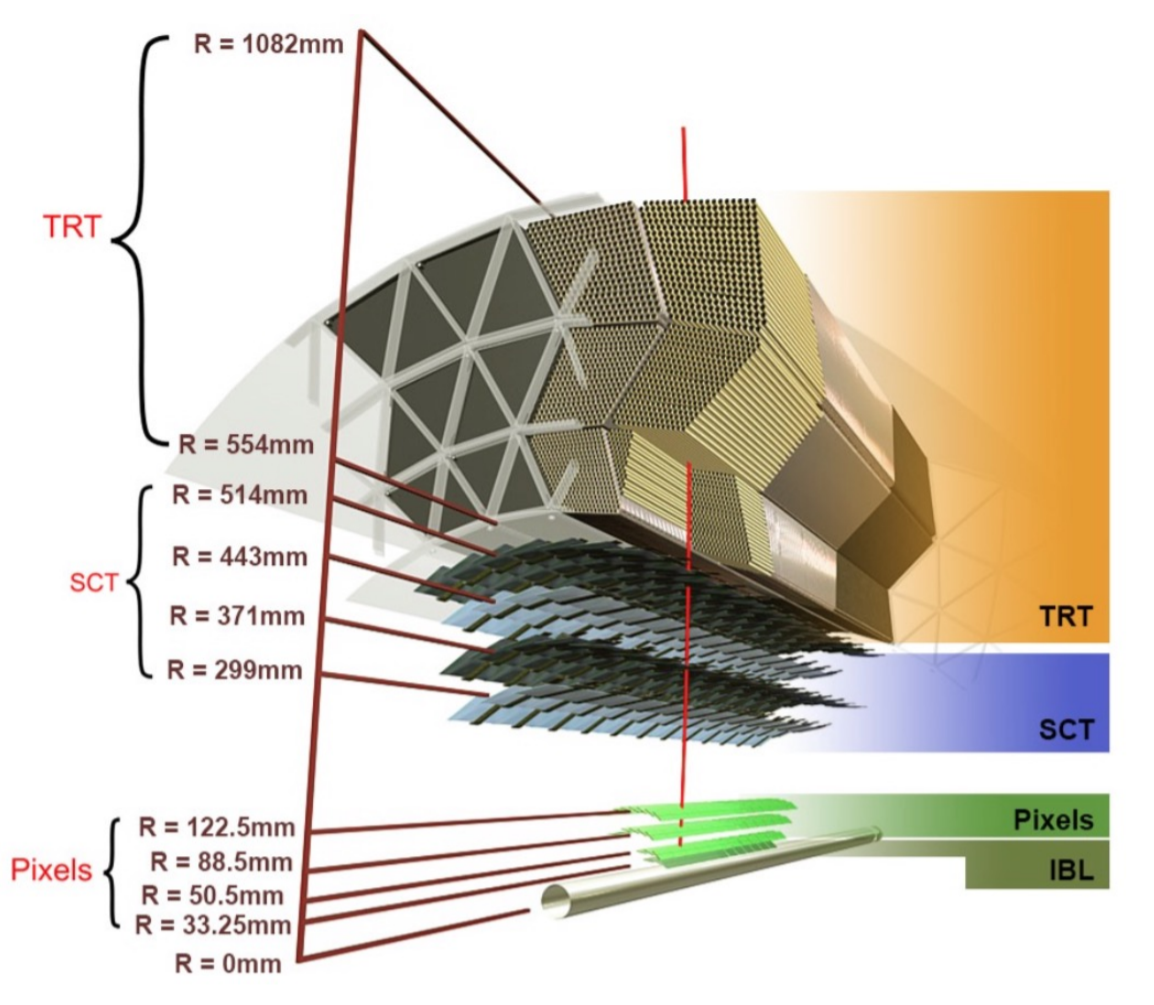
\includegraphics[width=0.7\textwidth]{figures/Simulation/track_ID.png}
  \caption{Cut-away view of the ATLAS inner detector.}
  \label{fig:track_ID}
\end{figure}

For inside-out tracking, it exploits the high granularity of the pixel and SCT detectors to discover prompt tracks originating from the interaction point.
In first step, the track seeds are formed by combining the information of space-points in the three pixel layers and the first SCT layer.
Then, these seeds are extended throughout the SCT to build track candidates.
After that, these candidates are fitted with some quality cuts applied to remove the outlier clusters, reject the fake tracks and resolve ambiguities in the cluster-to-track association.
The selected tracks are then further extended to TRT, and refitted with the full information from pixel, SCT and TRT detectors.

Another complementary approach, outside-in, searches for unused track segments start from TRT instead.
These segments are then extended into the SCT and pixel detectors to improve the tracking efficiency for secondary tracks from decays of long-lived particles or conversions.

\textbf{Muon spectrometer track}

First of all, the MS track reconstruction~\cite{Aad:2016jkr} searches for hit patterns inside muon chambers and forms the corresponding segments.
The Hough transform method~\cite{ILLINGWORTH198887} is used to search the hits lie on a certain trajectory in the bending plane in each MDT chamber and its nearby trigger chamber.
Then one can reconstruct the MDT segments by performing a linear fit to the hits found in each layer.
In the meantime, the hits informations from RPC or TGC can used to measure the coordinate orthogonal to the bending plane.
And the segments of CSC can be reconstructed using a separate combinatorial search in the $\eta$ and $\phi$ detector planes.

Then by fitting the hits informations from segments in different subsystems together, one can built the muon track candidates.
The reconstruction makes use of the algorithm by performing a segment-seeded combinatorial search, which starts by using the segments reconstructed in the middle layers of the detector where more trigger hits are available as seeds.
The search is then extended to use the segments as seeds from the inner and outer layers.
The segments are firstly selected based on criteria such as hit multiplicity and fit quality, and then matched using their relative positions and angles.
To build a track, at least two matching segments are required, except in the barrel-endcap transition region where a single high-quality segment can be used.
At beginning, one segment can be used to build more than one track candidates.
But then, an overlap removal algorithm is adopted to select the best assignment to one single track, or decide whether allows the certain segment to be shared between two tracks.

The hits associated with track candidates are then fitted using a global $\chi^{2}$ fit.
The algorithm accepts the track candidate if its fitting $\chi^{2}$ passes the required value.
Hits with large contribution to $\chi^{2}$ are removed and the track fit is repeated.
In addition, the algorithm performs a hit recovery procedure looking for additional hits consistent with the candidate trajectory, and the track candidate is refit if additional hits are found.
